\documentclass[9pt]{beamer}
\usetheme{TUDOplain}
% workaround: provide commands not defiend by all bibtex styles
\providecommand{\btxandlong}{und}
\providecommand{\newblock}{}

\usepackage{pgfpages}
\setbeameroption{hide notes}

% link for how to present on mac with skim:
% https://gist.github.com/andrejbauer/ac361549ac2186be0cdb

% sourcing images
\providecommand{\source}{\\ \footnotesize \tugreen{Source:} \footnotemark}
\providecommand{\sourcefix}[1]{\\ \footnotesize \tugreen{Source:} [#1]}

\renewcommand{\caption}[1]{\\ \footnotesize{\captiongrey{#1}}}

\usepackage[english]{babel}
\usepackage[style=authortitle]{biblatex}
\addbibresource{../bibliography.bib}

% reformat footnotes very plain
\makeatletter
\renewcommand\@makefnmark{%
[\@thefnmark]}
\renewcommand\@makefntext[1]{%
  \noindent\tiny [\@thefnmark] #1}
\makeatother
% command for citing
\providecommand{\fcite}[1]{\footcite{#1}}
%

% basic utils
\usepackage[utf8]{inputenc}
\usepackage{enumerate}
\usepackage{graphicx}
\graphicspath{{../images/}}

\AtBeginSection[]{
  \begin{frame}
  \note[item]{placeholder}
  \vfill
  \centering
  \begin{beamercolorbox}[sep=8pt,center,shadow=true,rounded=true]{title}
    \usebeamerfont{title}\insertsectionhead\par%
  \end{beamercolorbox}
  \vfill
  \end{frame}
}

\usepackage{ifthen}
\usepackage{calc}
\usepackage{amsmath,amsfonts,amssymb}
\setbeamertemplate{navigation symbols}{}
%\setbeamertemplate{footline}{}
%\setbeamertemplate{footline}[frame number]{}
\setbeamertemplate{footline}{\small \vspace{-1ex} \vbox{ \insertframenumber /\inserttotalframenumber}}
%\setbeamertemplate{footline}{\fontsize{7pt}{7pt}\selectfont \vspace{-1ex} \vbox{ \insertframenumber /\inserttotalframenumber}}

\author{Matthias Jakobs}
\title{End-to-end Human Activity Recognition framework on Complex Video Datasets \\ Final presentation}
\date{\today}
\institute[TU Dortmund]{Pattern Recognition In Embedded Systems,\\ Department of Computer Science \\ LS XII, Technische Universität Dortmund}
%
% frame command
\newenvironment{myframe}[1][]{%
\begin{frame}%
\frametitle{#1}
% start footnote numbers with 1
\setcounter{footnote}{0}


}{%
\end{frame}%
}

\begin{document}
\begin{frame}

\titlepage

\end{frame}

\section{Motivation}
\begin{myframe}[Motivation]
    \begin{columns}[T]
        \begin{column}{.45\textwidth}
            \begin{itemize}
                \item Often: Human Activity Recognition approached separately from pose estimation
                \item Pose is used for HAR, but not learned jointly.
                \begin{itemize}
                    \item Shown to be very important feature \footnotemark
                \end{itemize}
                \item Idea: Both can benefit from each other
                \item Luvizon et al. \footnotemark~ propose approach for jointly learning both
            \end{itemize}
        \end{column}
        \footnotetext[1]{\cite{jhuang_towards_2013}}
        \footnotetext[2]{\cite{luvizon_2d/3d_2018}}
        \footnotetext[3]{\cite{reining_towards_2018}}
        \begin{column}{.45\textwidth}
            \begin{figure}
                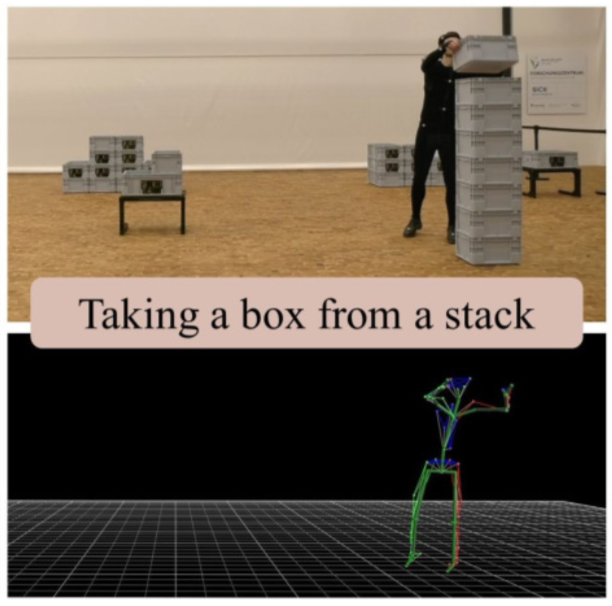
\includegraphics[width=.99\textwidth]{skeleton_har_example.png}
                \sourcefix{3}
            \end{figure}
        \end{column}
    \end{columns}
\end{myframe}

\tableofcontents

\section{Method}

\begin{myframe}[Method - Overview]
	\begin{columns}[T]
        \begin{column}{.45\textwidth}
            \begin{itemize}
                \item \textbf{Multitask Deep HAR}\footnotemark
                \begin{itemize}
                    \item Jointly train pose and action recognition
                    \item Pre-train pose estimation part, then fine-tune end-to-end
                    \item \textit{Soft-argmax}\footnotemark~makes end-to-end learning possible
                \end{itemize}
            \end{itemize}
        \end{column}
        \footnotetext[1]{\cite{luvizon_2d/3d_2018}}
        \footnotetext[2]{\cite{luvizon_human_2017}}
        \begin{column}{.45\textwidth}
            \begin{figure}
                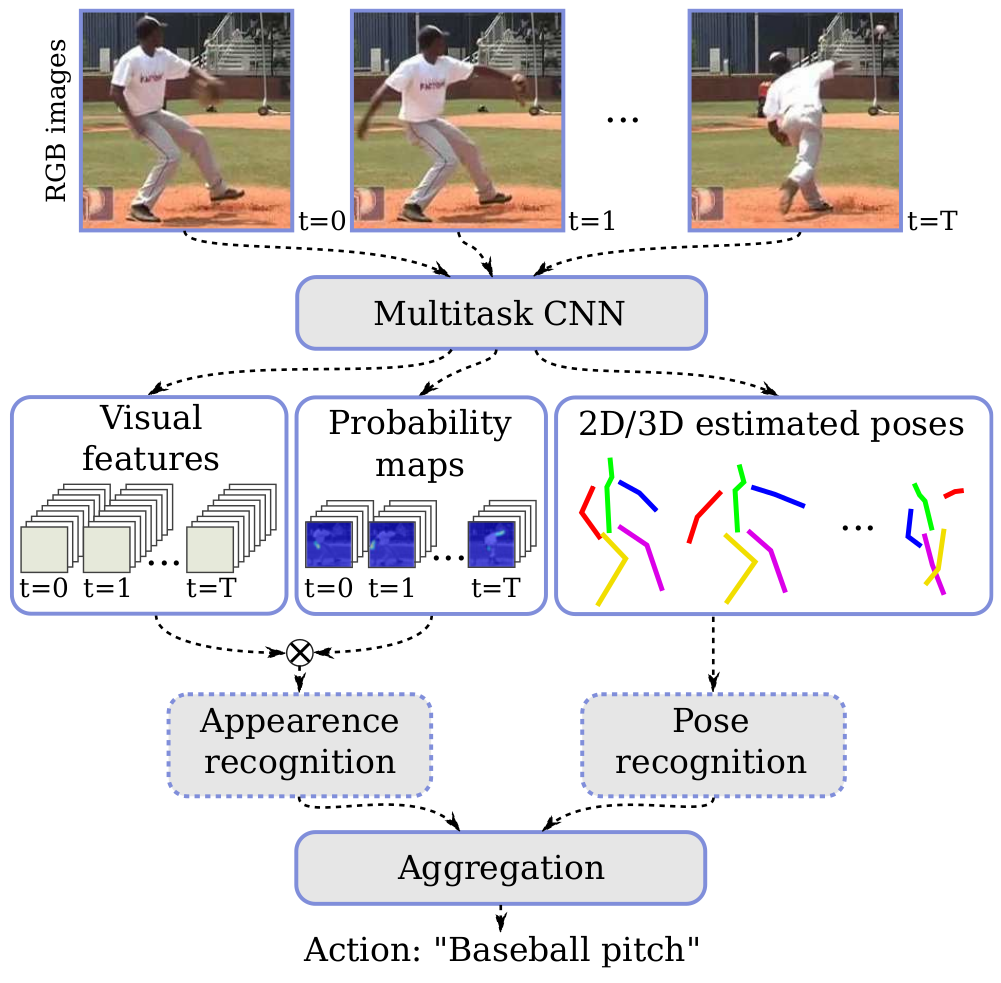
\includegraphics[width=.99\textwidth]{endtoend-concept.png}
                \sourcefix{1}
                %\caption{Complete network pipeline.}
            \end{figure}
        \end{column}
        \end{columns}
    \end{myframe}

\begin{myframe}[Method - Softargmax]
	\begin{columns}[T]
        \begin{column}{.45\textwidth}
            \begin{itemize}
                \item According to authors: Postprocessing necessary
                \item Propose \textbf{Soft-argmax} \footnotemark ~ in previous work
                \item Computes expectations on probability maps
                \item Fully differentiable
            \end{itemize}
        \end{column}
        \footnotetext[1]{\cite{luvizon_human_2017}}
        \footnotetext[2]{\cite{luvizon_2d/3d_2018}}
        \begin{column}{.45\textwidth}
            \begin{figure}
                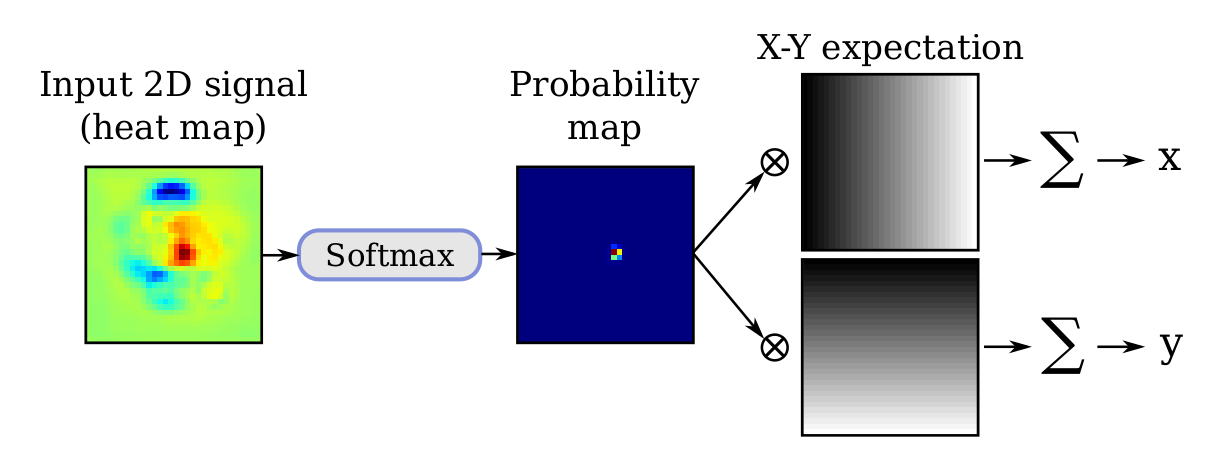
\includegraphics[width=.99\textwidth]{softargmax.png}
                \sourcefix{1}
                %\caption{Complete network pipeline.}
            \end{figure}
        \end{column}
	\end{columns}
\end{myframe}

% \begin{myframe}[Method - Architecture]
%     \begin{columns}[T]
%         \begin{column}{.45\textwidth}
%             \begin{itemize}
%                 \item \textit{Feature Extractor - Stem}
%                 \begin{itemize}
%                     \item Based on Inception v4 \footnotemark
%                     \item Implicit: Batch normalization and ReLU activation
%                     \item Uses \textbf{Depthwise separate convolutional layer}\footnotemark\footnotemark
%                     \begin{itemize}
%                         \item Used when high number of filters needed
%                         \item Needs fewer parameters
%                         \item Needs fewer matrix multiplications
%                     \end{itemize}
%                 \end{itemize}
%             \end{itemize}
%         \end{column}
%         \begin{column}{.45\textwidth}
%             \begin{figure}
%                 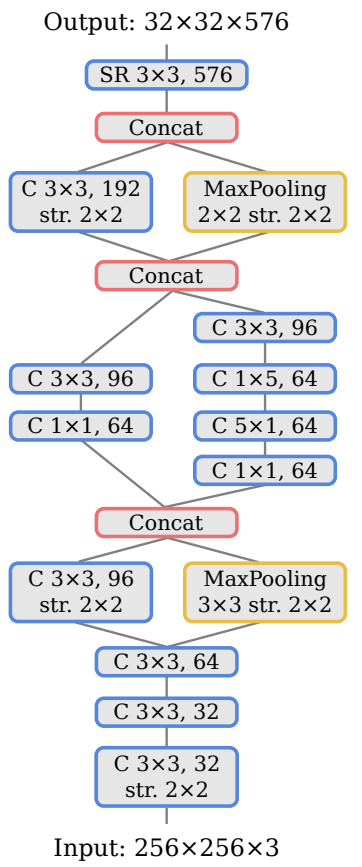
\includegraphics[width=.45\textwidth]{luvizon_stem.png}
%                 \sourcefix{4}
%             \end{figure}
%         \end{column}
% 	\end{columns}
%     \footnotetext[1]{\cite{szegedy_inception-v4_2017}}
%     \footnotetext[2]{\cite{sifre_rigid-motion_2014}}
%     \footnotetext[3]{\cite{chollet_xception:_2017}}
%     \footnotetext[4]{\cite{luvizon_2d/3d_2018}}
% \end{myframe}

\begin{myframe}[Method - Pose estimator]
    \begin{itemize}
        \item Features $\rightarrow$ prediction block
        \item Input and output dimensions identical
        \item Intermediate results via Soft-argmax function
    \end{itemize}
    \begin{figure}
        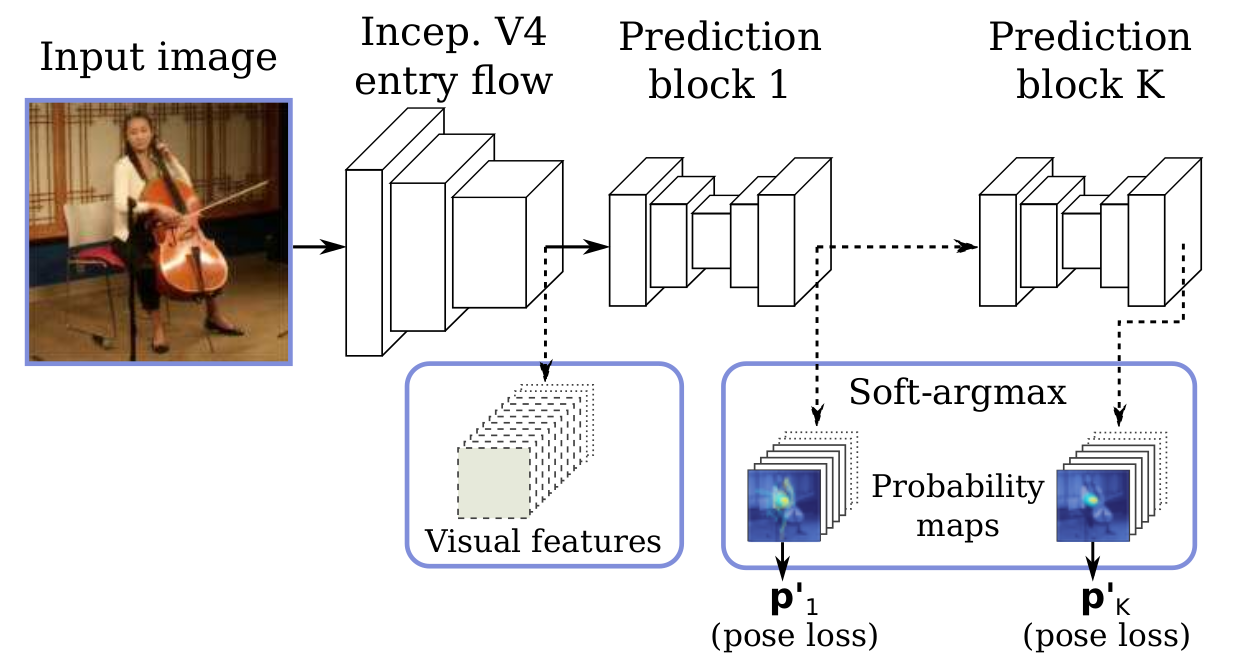
\includegraphics[width=.80\textwidth]{multitask-part.png}
        \sourcefix{1}
        \caption{Pose estimation pipeline. Notice the intermediate results after each prediction block.}
    \end{figure}
    \footnotetext[1]{\cite{luvizon_2d/3d_2018}}
\end{myframe}

\begin{myframe}[Method - Pose Model]
	\begin{columns}[T]
        \begin{column}{.45\textwidth}
            \begin{itemize}
                \item Two paths in the network for action recognition
                \item \textit{Pose Model}
                \begin{itemize}
                    \item Arrange joint values over time in 2D matrix (\textit{pose cube})
                    \item Action heatmaps
                    \begin{itemize}
                        \item Through softmax: action probabilities
                    \end{itemize}
                \end{itemize}
            \end{itemize}
        \end{column}
        \begin{column}{.45\textwidth}
            \begin{figure}
                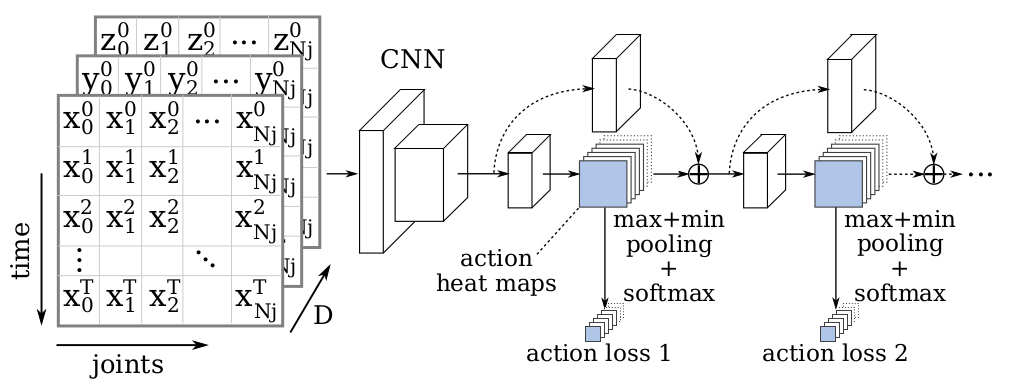
\includegraphics[width=.99\textwidth]{jointsovertime.png}
                \sourcefix{1}
            \end{figure}
        \end{column}
	\end{columns}
    \footnotetext[1]{\cite{luvizon_2d/3d_2018}}
\end{myframe}

% \begin{myframe}[Method - Pose Model]
%     \begin{figure}
%         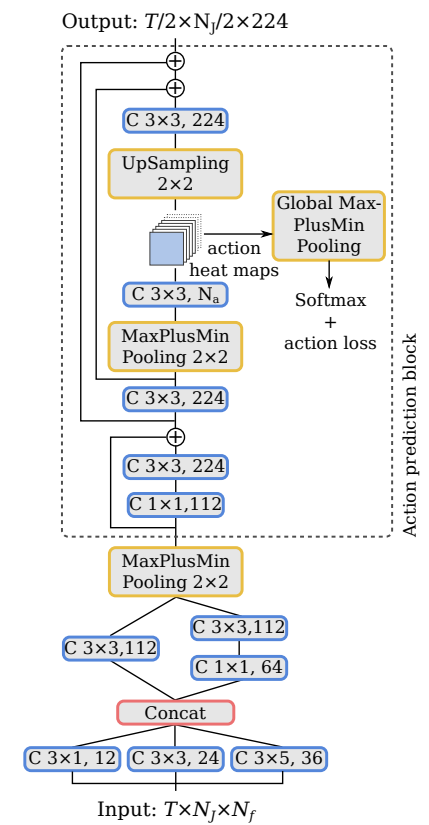
\includegraphics[width=.30\textwidth]{luvizon_actionrecognitionblock.png}
%         \sourcefix{1}
%     \end{figure}
%     \footnotetext[1]{\cite{luvizon_2d/3d_2018}}
% \end{myframe}

\begin{myframe}[Method - Visual Model]
    	\begin{columns}[T]
        \begin{column}{.45\textwidth}
            \begin{itemize}
                \item \textit{Visual Model}
                \begin{itemize}
                    \item Combination of visual features and joint probability maps
                    \item Then: Simple feature extraction on \textit{appearance cube}
                    \item Array of action precition blocks as seen before
                \end{itemize}
                \item \textit{Aggregation}
                \begin{itemize}
                    \item Combine Pose Model and Visual Model results for final result
                    \item \textit{Categorical cross-entropy}
                \end{itemize}
            \end{itemize}
        \end{column}
        \begin{column}{.45\textwidth}
            \begin{figure}
                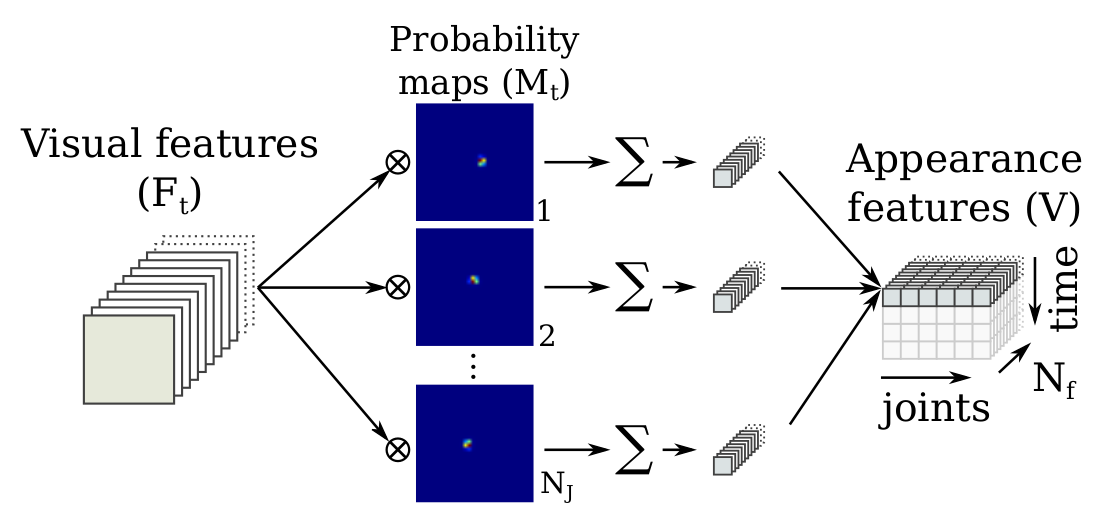
\includegraphics[width=.99\textwidth]{appearance-features.png}
                \sourcefix{1}
            \end{figure}
            \begin{figure}
                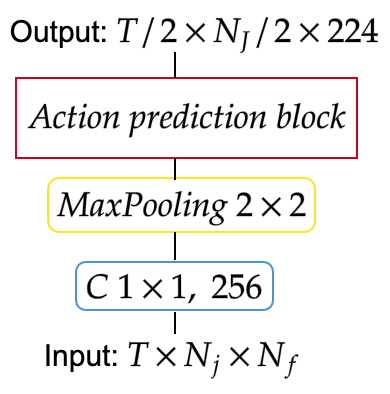
\includegraphics[width=.50\textwidth]{luvizon_appearancebasedaction.png}
            \end{figure}
        \end{column}
	\end{columns}
    \footnotetext[1]{\cite{luvizon_2d/3d_2018}}
\end{myframe}

% \begin{myframe}[Method - Extensions]
%     \begin{itemize}
%         \item Reimplementation in PyTorch \fcite{paszke_automatic_2017}
%         \begin{itemize}
%             \item Evaluate against JHMDB \fcite{jhuang_towards_2013}
%         \end{itemize}
%         \item Experimentation
%         \begin{itemize}
%             %\item Better incorporation of temporal dimension \fcite{pavllo_3d_2019}
%             \item Ablation study to determine the choice of certain parameters
%             \item Combined loss function of pose and action for \emph{real} end-to-end training
%             \item Different representation of temporal information (next slide)
%             \begin{itemize}
%                 \item Idea: Use for IMU time series data as presented in \footnotemark
%             \end{itemize}
%         \end{itemize}
%     \end{itemize}
%     \footnotetext[3]{\cite{reining_towards_2018}}
% \end{myframe}

% \begin{myframe}[Method - Different temporal representation]
%     \begin{figure}
%         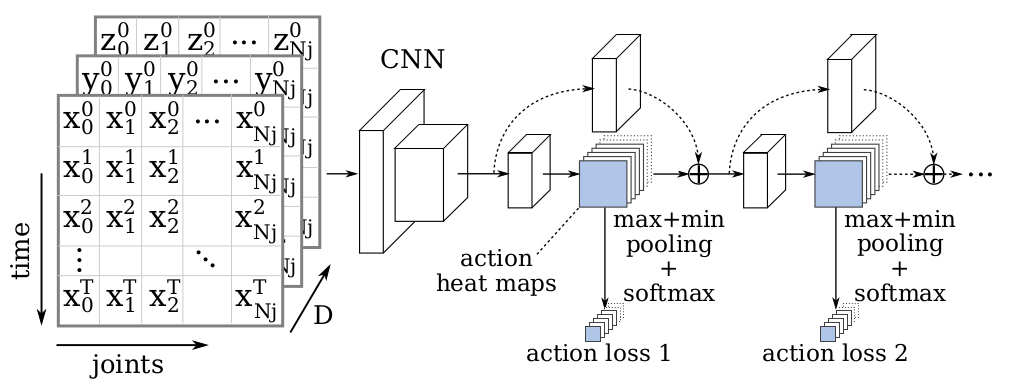
\includegraphics[width=.65\textwidth]{jointsovertime.png}
%         \caption{Approach used by \footnotemark. Convolution over all sensors at once. \sourcefix{1}}
%     \end{figure}
%     \begin{figure}
%         \includegraphics[width=.65\textwidth]{sensor-time.png}
%         \caption{Impression of pixel coordinates of joints over time \source}
%     \end{figure}
%     \footnotetext[1]{\cite{luvizon_2d/3d_2018}}
%     \footnotetext[2]{\url{https://avtech.com/articles/wp-content/uploads/2015/06/Intro.-Pic.png}}
% \end{myframe}

\section{Datasets}
\begin{myframe}[2D Pose Datasets]
  \note[item]{placeholder}
  \begin{columns}[T]
      \begin{column}{.48\textwidth}
          \begin{itemize}
              \item \textbf{MPII Human Pose\footnotemark}
              \begin{itemize}
                  \item 40,000 annotated images
                  \begin{itemize}
                      \item 2D pose
                      \item Head size
                      \item Center of Person bounding box
                  \end{itemize}
                  \item Single and multi person
                  \item Over 401 different activities from YouTube videos
                  \item Test image predictions to be send to Max Planck institute
              \end{itemize}
          \end{itemize}
      \end{column}
      \footnotetext[1]{\cite{andriluka_2d_2014}}
      \begin{column}{.48\textwidth}
          \begin{figure}
              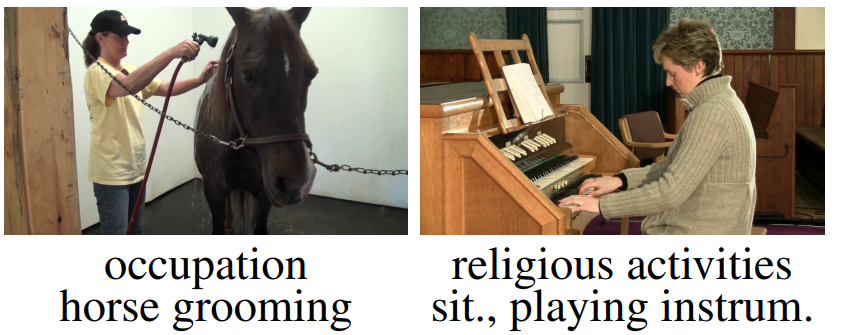
\includegraphics[width=0.99\textwidth]{mpii.png}
              \sourcefix{1}
          \end{figure}
      \end{column}
  \end{columns}
\end{myframe}

\begin{myframe}[Action Recognition Datasets]
  \begin{columns}[T]
      \begin{column}{.48\textwidth}
          \vspace{20px}
          \begin{itemize}
              \item \textbf{Penn Action\footnotemark}
              \begin{itemize}
                  \item 2,400 video clips of 15 actions ($149.355$ total frames)
                  \item Limited number of actions (mainly sport)
                  \item Literature ``solved'' this dataset
              \end{itemize}
          \end{itemize}
      \end{column}
      \footnotetext[1]{\cite{zhang_actemes_2013}}
      \begin{column}{.48\textwidth}
          \begin{figure}
              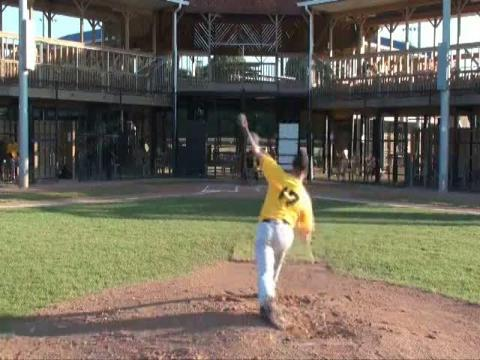
\includegraphics[height=45px]{pa-01.jpg}
              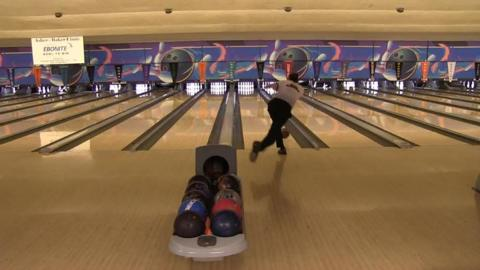
\includegraphics[height=45px]{pa-02.jpg}
              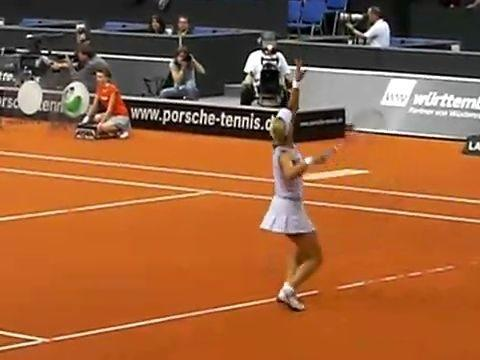
\includegraphics[height=45px]{pa-03.jpg}
              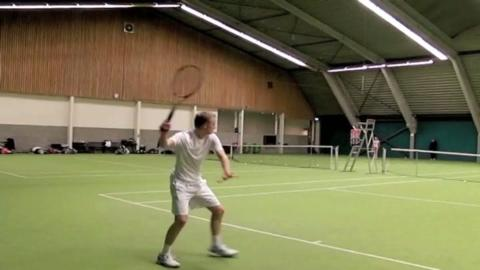
\includegraphics[height=45px]{pa-04.jpg}
              \source
          \end{figure}
      \end{column}
  \end{columns}
  \footnotetext[2]{\url{https://upenn.app.box.com/v/PennAction}}
\end{myframe}

\begin{myframe}[Action Recognition Datasets]
  \begin{columns}[T]
      \begin{column}{.48\textwidth}
          \begin{itemize}
              \item \textbf{JHMDB\footnotemark}
              \begin{itemize}
                  \item Fully-annotated subset of HMDB
                  \begin{itemize}
                      \item 2D pose
                      \item Subject segmentation maps
                      \item Optical flow
                  \end{itemize}
                  \item 928 clips of 21 actions ($31.838$ total frames)
                  \begin{itemize}
                      \item More diverse than Penn Action in terms of actions
                  \end{itemize}
              \end{itemize}
          \end{itemize}
      \end{column}
      \footnotetext[1]{\cite{jhuang_towards_2013}}
      \begin{column}{.48\textwidth}
          \begin{figure}
              \includegraphics[height=.55\textheight]{jhmdb.png}
              \centering
              \source
          \end{figure}
      \end{column}
  \end{columns}
  \footnotetext[2]{\url{http://jhmdb.is.tue.mpg.de/puppet_tool}}
\end{myframe}

\section{Experiments}

\begin{myframe}[Determining Soft-argmax accuracy]
    \begin{itemize}
        \item Qualitative evaluation
        \begin{itemize}
            \item Place $2D$ gaussian with covariance $c$ at each $(i,j)$ position
            \item Regress coordinates
            \item Yellow: Regressed coordinate accurate within $1$ pixel for each dimension
            \begin{itemize}
                \item Threshold to account for rounding error
            \end{itemize}
        \end{itemize}
    \end{itemize}
    \begin{figure}
        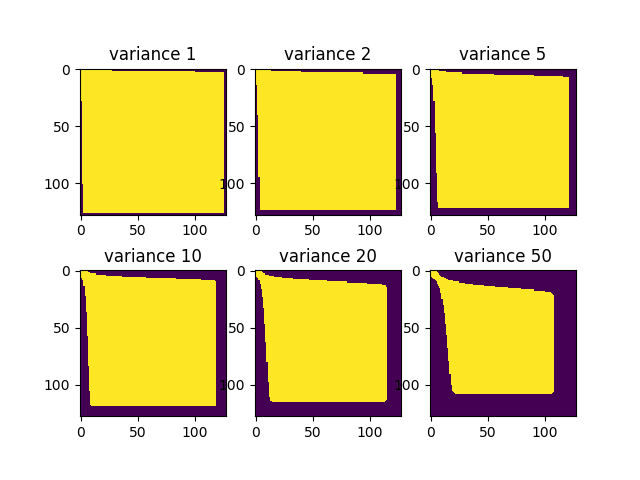
\includegraphics[height=.60\textheight]{softargmax_variance_test.png}
        \centering
    \end{figure}    
\end{myframe}

\begin{myframe}[Determining Soft-argmax accuracy]
    \begin{itemize}
        \item Quantitative evaluation
        \begin{itemize}
            \item Place $2D$ gaussian with covariance $c$ at each joint position $(i,j)$
            \item Regress coordinates as before
            \item Taken from $1000$ random validation images from MPII dataset
        \end{itemize}
    \end{itemize}
    \begin{table}[]
        \centering
        \scalebox{0.90}{%
        \begin{tabular}{|l|l|l|l|l|l|l|}
        \hline
        threshold & \textbf{$c=1$} & \textbf{$c=2$} & \textbf{$c=5$} & \textbf{$c=10$} & \textbf{$c=20$} & \textbf{$c=50$} \\ \hline
        $1$ & 93.137 & 93.123 & 93.069 & 92.988 & 92.811 & 92.201 \\ \hline
        $2$ & 99.952 & 99.931 & 99.843 & 99.741 & 99.469 & 98.598 \\ \hline
        $3$ & 99.959 & 99.945 & 99.891 & 99.809 & 99.639 & 99.054 \\ \hline
        $4$ & 99.959 & 99.952 & 99.911 & 99.829 & 99.700 & 99.197 \\ \hline
        \end{tabular}}
    \end{table}    
\end{myframe}

\begin{myframe}[Recreate experiments - Meassurements]
    % TODO: Cite all this
    \begin{itemize}
        \item 2D Pose estimation
        \begin{itemize}
            \item \textit{Probability of Correct Keypoints} with regards to head size (\textit{PCKh})
            \begin{itemize}
                \item Meassure distance between ground truth keypoint and estimation
                \item If smaller than ($\alpha \cdot \text{head bbox size}$): correctly estimated
                \item Used for highly articulated poses
                \item In literature: $\alpha \in \{0.2, 0.5\}$
            \end{itemize}    
            \item \textit{PCK} with regards to subject bounding box
            \begin{itemize}
                \item Problem with highly articulated poses
                \item Used whenever no head size given
                \item Can be computed from all datasets used
                \item $\alpha = 0.2$ used in literature
            \end{itemize}
        \end{itemize}
        \item Action recognition
        \begin{itemize}
            \item Simple accuracy meassurement in literature
            \item $F_1$ meassure not needed since all datasets are balanced w.r.t. classes
            \item Single and Multi Clip accuracy
        \end{itemize}
    \end{itemize}
\end{myframe}

\begin{myframe}[Recreate experiments - 2D Pose estimation]
    \begin{itemize}
        \item Recreate results for using different parameters
        \item \textit{Validation accuracies}
        \item Evaluate significance using randomization test
        \begin{itemize}
            \item Improvement only statistically significant between $2$ and $8$ blocks (with significance level $0.05$)
            \item Significantly worse in comparison to authors
        \end{itemize}
    \end{itemize}
    \begin{figure}
        \begin{table}[]
            \small
            \centering
            \scalebox{0.90}{%
            \begin{tabular}{ll}
                \begin{tabular}{|l|l|c|c|}
                    \hline
                    \textbf{blocks} & \textbf{context}  & \textbf{PCKh @ 0.5} & \textbf{p-values} \\ \hline
                    \begin{tabular}{@{}c@{}} 2 \\ 2 \end{tabular} & \begin{tabular}{@{}c@{}} 0 \\ 2 \end{tabular} & \begin{tabular}{@{}c@{}} 84.15 \\ 84.01  \end{tabular} & 0.85  \\ \hline
        
                    \begin{tabular}{@{}c@{}} 4 \\ 4 \end{tabular} & \begin{tabular}{@{}c@{}} 0 \\ 2 \end{tabular} & \begin{tabular}{@{}c@{}} 85.78 \\ 85.64  \end{tabular} & 0.85  \\ \hline
        
                    \begin{tabular}{@{}c@{}} 8 \\ 8 \end{tabular} & \begin{tabular}{@{}c@{}} 0 \\ 2 \end{tabular} & \begin{tabular}{@{}c@{}} 86.71 \\ \textbf{87.00}  \end{tabular} & 0.73  \\ \hline
        
                    \begin{tabular}{@{}c@{}} 2 \\ 4 \end{tabular} & \begin{tabular}{@{}c@{}} 0 \\ 0 \end{tabular} & \begin{tabular}{@{}c@{}} 84.15 \\ 85.78  \end{tabular} & 0.074  \\ \hline
        
                    \begin{tabular}{@{}c@{}} 2 \\ 4 \end{tabular} & \begin{tabular}{@{}c@{}} 2 \\ 2 \end{tabular} & \begin{tabular}{@{}c@{}} 84.01 \\ 85.64  \end{tabular} & 0.076  \\ \hline
        
                \end{tabular}
                \begin{tabular}{|l|l|c|c|}
                    \hline
                    \textbf{blocks} & \textbf{context}  & \textbf{PCKh @ 0.5} & \textbf{p-values} \\ \hline
        
                    \begin{tabular}{@{}c@{}} 4 \\ 8 \end{tabular} & \begin{tabular}{@{}c@{}} 0 \\ 0 \end{tabular} & \begin{tabular}{@{}c@{}} 85.78 \\ 86.71  \end{tabular} & 0.31  \\ \hline
        
                    \begin{tabular}{@{}c@{}} 4 \\ 8 \end{tabular} & \begin{tabular}{@{}c@{}} 2 \\ 2 \end{tabular} & \begin{tabular}{@{}c@{}} 85.64 \\ \textbf{87.00}  \end{tabular} & 0.12  \\ \hline
        
                    \begin{tabular}{@{}c@{}} 2 \\ 8 \end{tabular} & \begin{tabular}{@{}c@{}} 0 \\ 0 \end{tabular} & \begin{tabular}{@{}c@{}} 84.15 \\ 86.71  \end{tabular} & \textbf{0.006}  \\ \hline
        
                    \begin{tabular}{@{}c@{}} 2 \\ 8 \end{tabular} & \begin{tabular}{@{}c@{}} 2 \\ 2 \end{tabular} & \begin{tabular}{@{}c@{}} 84.01 \\ \textbf{87.00}  \end{tabular} & \textbf{0.001}  \\ \hline
        
                    \begin{tabular}{@{}c@{}} 8 \\ 8* \end{tabular} & \begin{tabular}{@{}c@{}} 2 \\ 2* \end{tabular} & \begin{tabular}{@{}c@{}} 87.00 \\ 89.00*  \end{tabular} & \textbf{0.025}  \\ \hline
                \end{tabular}
            \end{tabular}}
        \end{table}
    \end{figure}
    * Validation results from \footnotemark
    \footnotetext[1]{\cite{luvizon_2d/3d_2018}}
\end{myframe}

\begin{myframe}[Recreate experiments - 2D pose estimation]
    \begin{itemize}
        \item \textit{Test accuracies}
        \begin{itemize}
            \item Large discrepancy most likely due to testing procedure
            \item $89\%$ validation accuracy vs. $91.2\%$ testing accuracy
        \end{itemize}
    \end{itemize}
    \begin{table}[]
        \centering
        \scalebox{0.85}{%
        \begin{tabular}{|l|l|l|l|l|l|l|l|l|c|}
            \hline
            &Head & Shoulder & Elbow & Wrist & Hip & Knee  & Ankle & Total & p-value \\ \hline
            %out recreation& 95.7  & 90.5  & 81.4  & 74.6  & 82.5  & 73.0 & 66.2 & 81.4 \\
            our recreation            & 96.1  & 92.5  & 83.8  & 78.2  & 84.5  & 77.2 & 71.5 & 84.1 & \\
            \footnotemark & 98.1  & 96.6  & 92.0  & 87.5  & 90.6  & 88.0 & 82.7 & 91.2 & \textbf{0.0}  \\ \hline
        \end{tabular}}
    \end{table}
    \footnotetext[1]{\cite{luvizon_2d/3d_2018}}
\end{myframe}

% \begin{myframe}[Recreate experiments - 2D pose estimation]
%     \begin{figure}
%         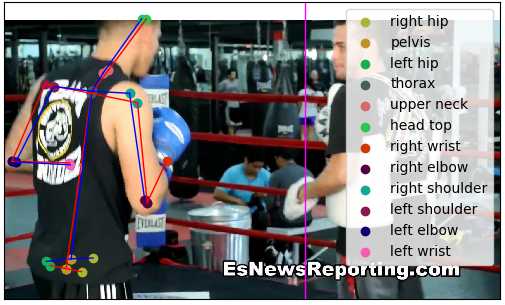
\includegraphics[height=.80\textheight]{mpii_8_positive.png}
%         \centering
%         \caption{\tugreen{Figure:} Positive example. Ground truth pose shown in red, estimated pose shown in blue.}
%     \end{figure}
% \end{myframe}

% \begin{myframe}[Recreate experiments - 2D pose estimation]
%     \begin{figure}
%         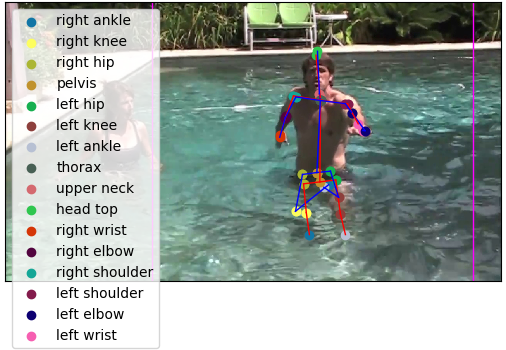
\includegraphics[height=.80\textheight]{mpii_8_negative.png}
%         \centering
%         \caption{\tugreen{Figure:} Negative example. Notice that the lower limbs are wrongly estimated due to the water.}
%     \end{figure}    
% \end{myframe}

\begin{myframe}[Recreate experiments - 2D pose estimation]
    \begin{figure}
        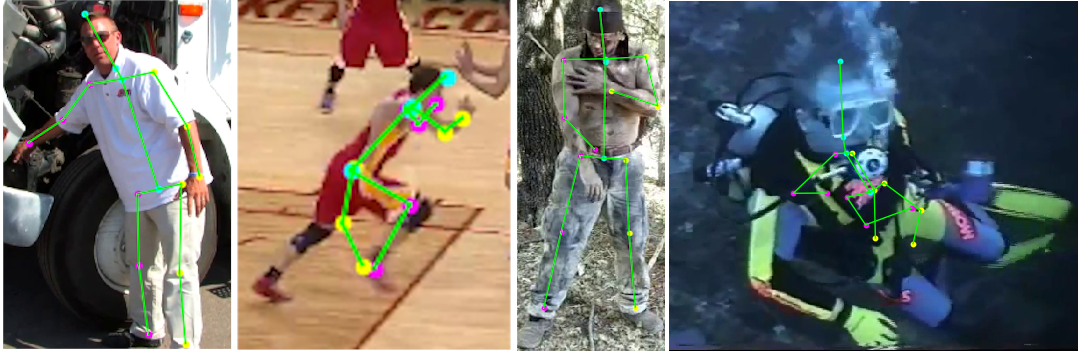
\includegraphics[width=.99\textwidth]{mpii_example_results.png}
        \centering
        %\caption{\tugreen{Figure:} Negative example. Notice that the lower limbs are wrongly estimated due to the water.}
    \end{figure}    
\end{myframe}


\begin{myframe}[Recreate experiments - HAR on Penn Action]
    \begin{columns}[T]
        \begin{column}{.48\textwidth}
            \begin{itemize}
                \item Pretrain pose estimator weights
                \item Mixed dataset of $25\%$ Penn Action and $75\%$ MPII
                \item Trained until validation accuracy plateaus
                \item Authors do not provide results for accuracies\footnotemark
                % \item First: Pose estimator is not fine-tuned, locked weights
                % \item Find validation plateau and then start fine-tuning with smaller learning rate
            \end{itemize}
            \vspace*{20px}
            \begin{table}[]
                \small
                \centering
                \begin{tabular}{|c|c|}
                \hline
                    \textbf{PCK @ 0.2} & \textbf{PCK @ 0.1} \\ \hline
                    80.26 & 59.28 \\ \hline
                \end{tabular}
                \caption{Test accuracies computed on Penn Action test dataset}
            \end{table}  
        \end{column}
        \begin{column}{0.45\textwidth}
            \begin{figure}
                \centering
                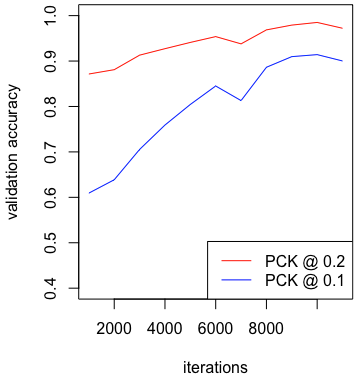
\includegraphics[width=0.95\textwidth]{pose_mixed_results.png}    
                \centering
            \end{figure}        
        \end{column}    
    \end{columns}    
    \footnotetext[1]{\cite{luvizon_2d/3d_2018}}
\end{myframe}

\begin{myframe}[Recreate experiments - HAR on Penn Action]
    \begin{itemize}
        \item Limbs on the right side of the body (from subject perspective) get estimated significantly better (with significance level of $0.05$)
    \end{itemize}
    \begin{table}[]
        \small
        \centering
        \scalebox{0.90}{%
        \begin{tabular}{|c|c|c|c|c|c|c|}
        \hline
            \textbf{Ankle (r)} & \textbf{Knee (r)}  & \textbf{Hip (r)} & \textbf{Hip (l)} & \textbf{Knee (l)} & \textbf{Ankle (l)}  & \textbf{Upper neck} \\ \hline 
            70.24 & 65.11 & 68.98 & 64.81 & 62.23 & 71.92 & 36.92 \\ \hline

            \textbf{Wrist (r)} & \textbf{Elbow (r)} & \textbf{Shoulder (r)} & \textbf{Shoulder (l)} & \textbf{Elbow (l)} & \textbf{Wrist (l)} & \textbf{Total}\\ \hline
            45.3 & 54.86  & 69.12 & 67.71 & 54.53 & 42.50 & 59.28 \\ \hline \hline
            
            \textbf{Arms (l)} & \textbf{Arms (r)} & \textbf{Arms (both)} & \textbf{Legs (l)} & \textbf{Legs (r)} & \textbf{Legs (both)} & \textbf{Upper body} \\ \hline
            \textit{54.92} & \textit{56.45} & 55.68 & \textit{66.34} & \textit{68.11} & 67.22 & 46.37\\ \hline
            
        \end{tabular}}
        \caption{Per joint accuracies of the pose estimator trained on mixed data}
        \label{tab:pose-mixed-perjoint}
    \end{table}    
\end{myframe}

\begin{myframe}[Recreate experiments - HAR on Penn Action]
    \begin{itemize}
        \item Pretrained weights of pose estimator initially frozen
        \item At blue line: Weights get unfrozen (after validation accuracy plateaus)
        \item Fine tuning results in worse validation accuracy
        \item Evaluation done on non-finetuned model
    \end{itemize}
    \begin{figure}[htb!]
        \centering
        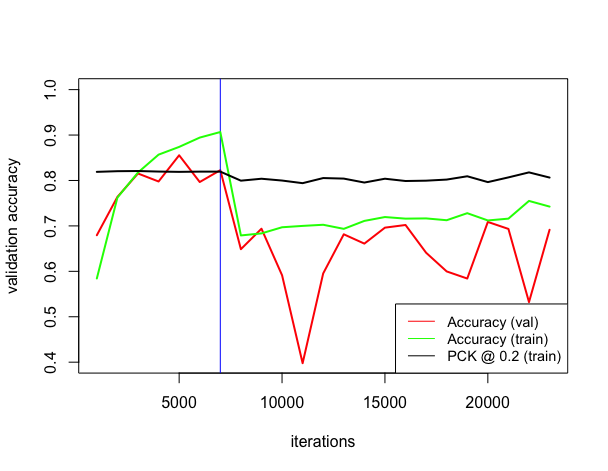
\includegraphics[width=0.8\textwidth]{har_pennaction_training.png}
    \end{figure}
\end{myframe}

\begin{myframe}[Recreate experiments - HAR on Penn Action]
    \begin{itemize}
        \item HAR accuracy significantly lower in comparison to \footnotemark[1]
        \item Pose estimator might achieve higher accuracy in author's work
        \item The authors do not provide training code
    \end{itemize}
    \begin{table}[]
        \small
        \centering
        \scalebox{0.90}{%
        \begin{tabular}{|c|c|c|}
        \hline
            \textbf{Single Clip accuracy} & \textbf{Multi Clip accuracy} & \footnotemark[1]\\ \hline
            79.56 & 81.66 & 97.40 \\ \hline
        \end{tabular}}
        \caption{Test accuracies in comparison to \footnotemark[1]}
        \label{tab:pennaction_test_results}
        \footnotetext[1]{\cite{luvizon_2d/3d_2018}}
    \end{table}
    
\end{myframe}

\begin{myframe}[Recreate experiments - HAR on Penn Action]
    \begin{itemize}
        \item Model is most uncertain with the class \textit{clean and jerk}.
        \begin{itemize}
            \item Contains similar poses to \textit{squats} and \textit{jumping jacks} classes, which might explain the confusion
            \item Better pose estimator might reduce the confusion
        \end{itemize}
    \end{itemize}
    \begin{figure}[htb!]
        \centering
        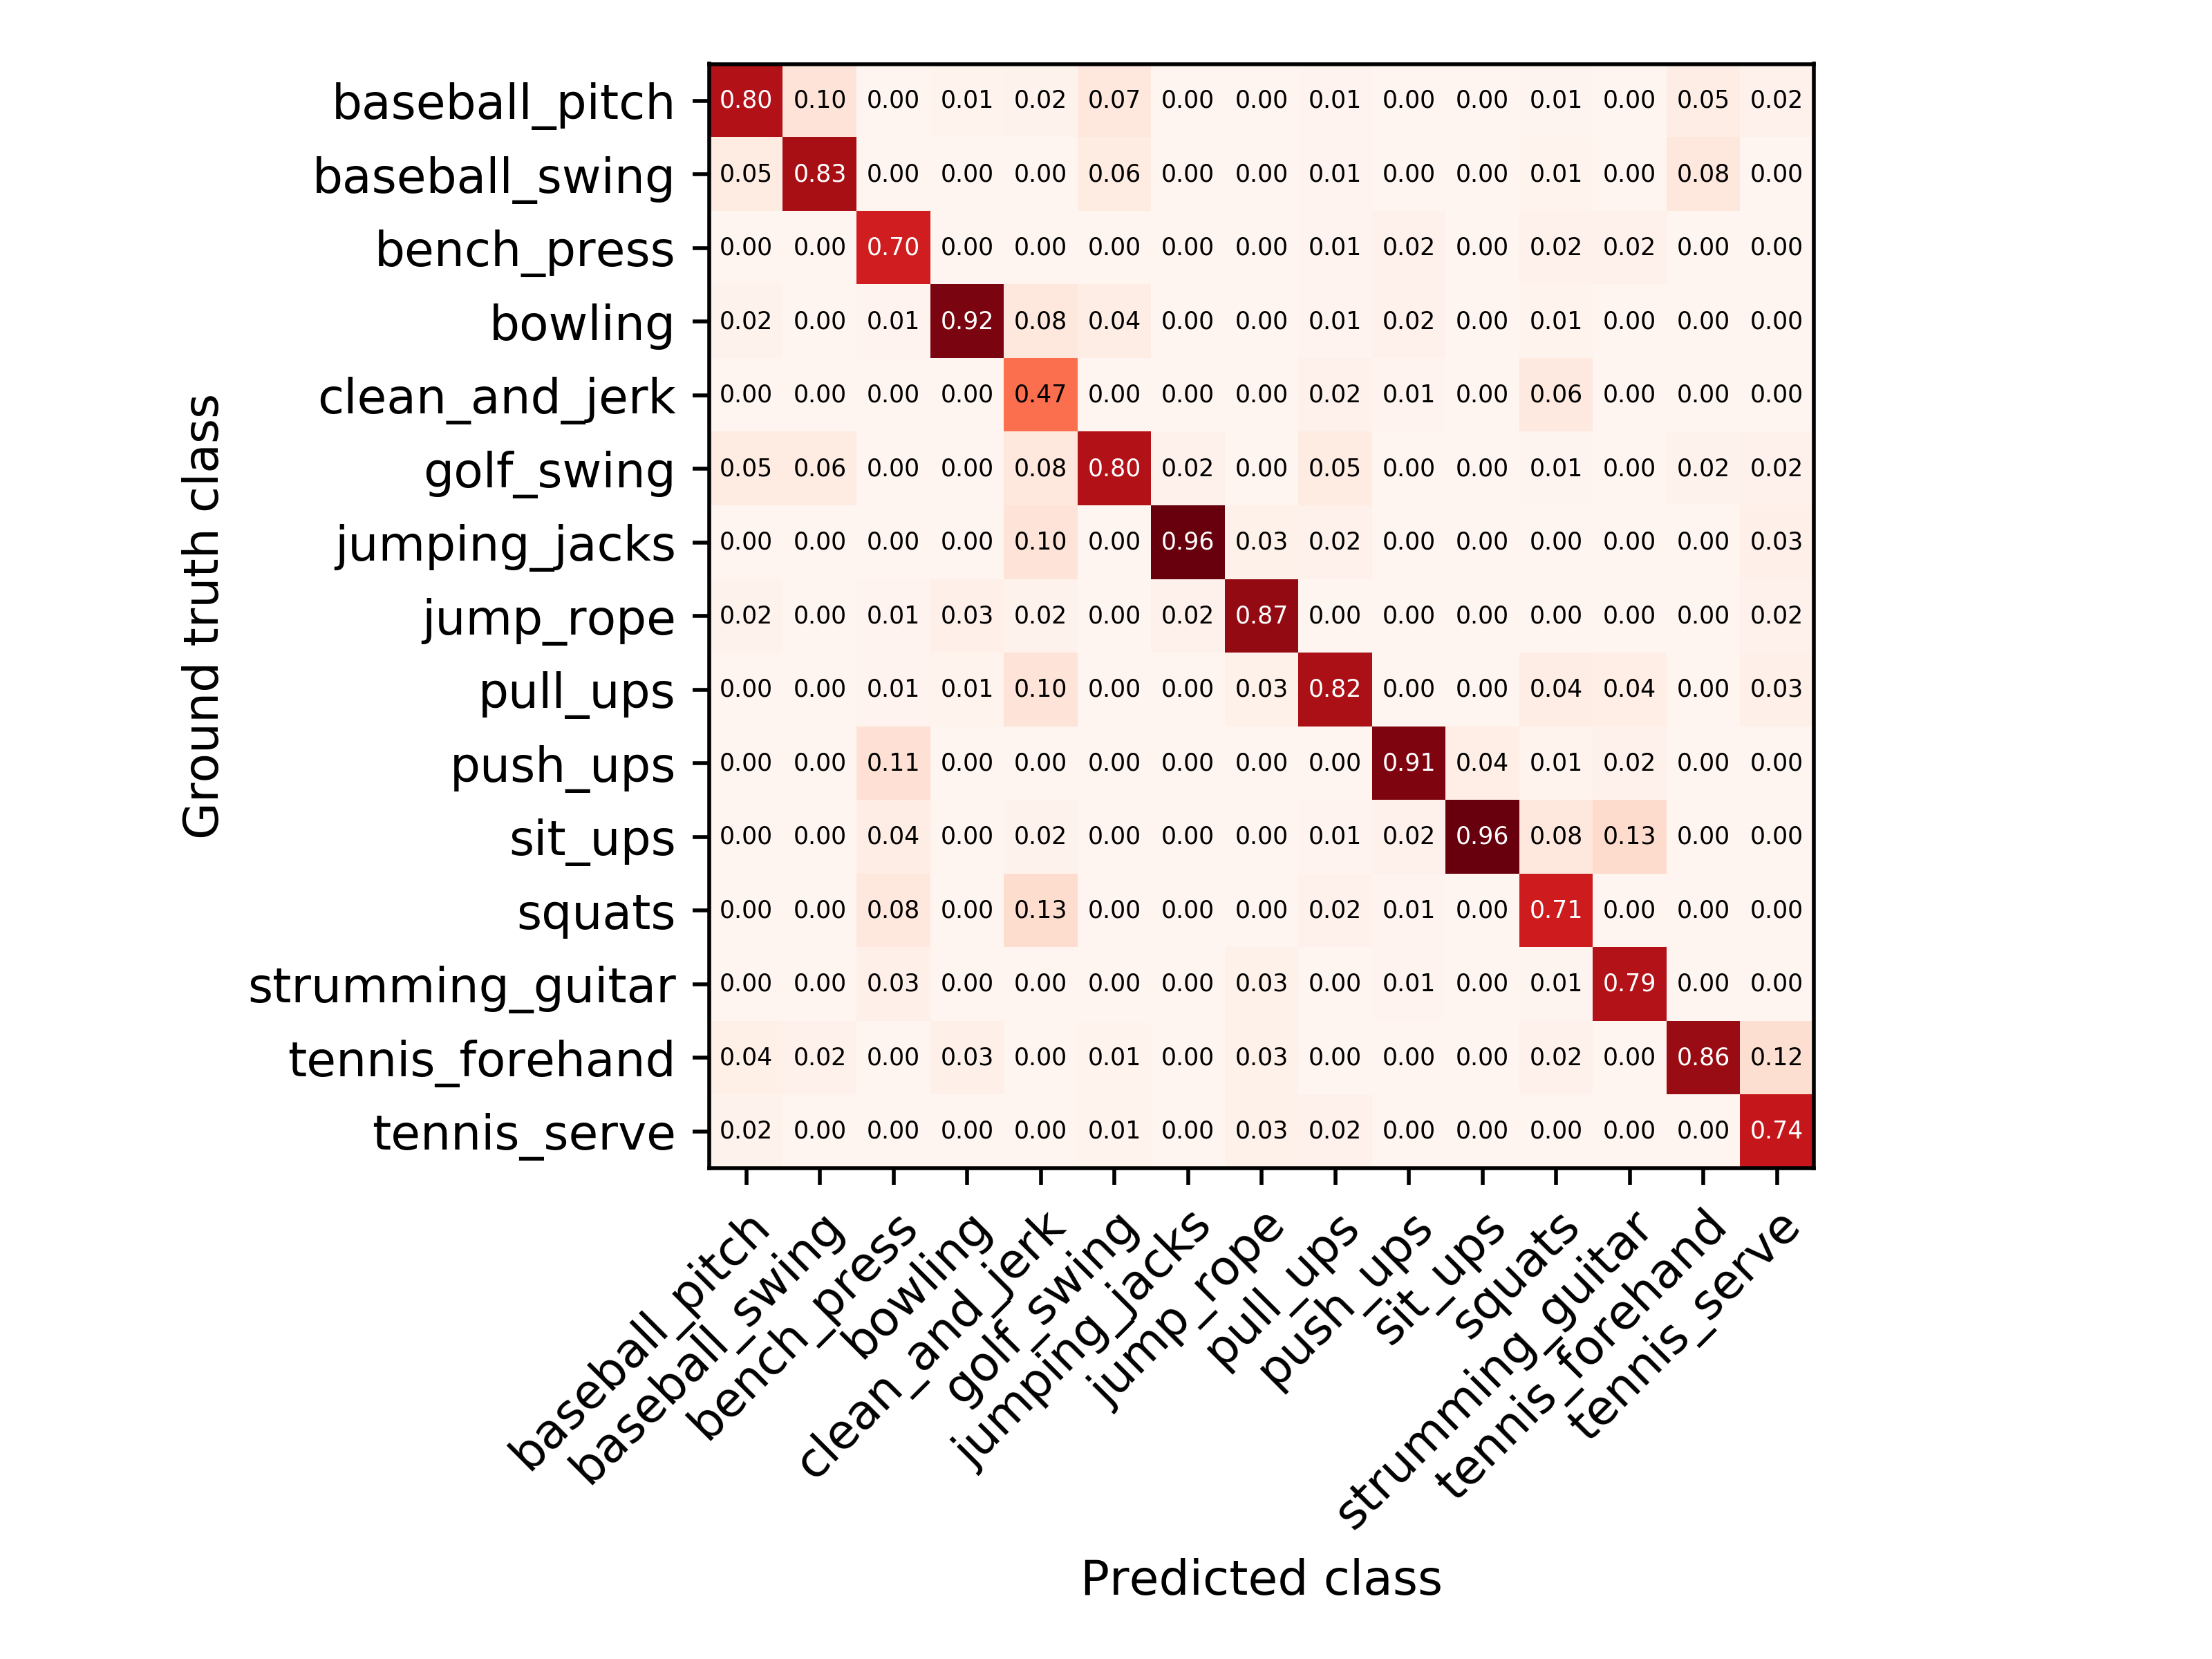
\includegraphics[width=0.85\textwidth]{confusion_matrix_pennaction.png}
        \caption{Confusion matrix of the Penn Action test set after training the HAR classifier. }
        \label{fig:cm-pennaction}
    \end{figure}
\end{myframe}

\begin{myframe}[2D pose estimation on JHMDB]
    \begin{itemize}
        \item Used ground truth bounding boxes as in \footnotemark
        \item Additionally: \textit{PCK} w.r.t. upper body size (\textit{PCKu})
        \item Dataset more challenging because of video artifacts
        \item Comparison: \footnotemark[2] achieve $81.6\%$ PCK @ $0.2$ and $68.7\%$ PCK @ $0.1$
        \item Unclear whether or not \footnotemark[2] use ground truth bounding box
        \item Per joint accuracy: Right side limbs better accuracy in comparison to left side limbs (as before)
    \end{itemize}
    \begin{table}[]
        \small
        \centering
        \scalebox{0.90}{%  
        \begin{tabular}{|l|c|c|c||c|c|c||c|c|c|}
        \hline
            & & & \textbf{p-value} & & & \textbf{p-value} & & & \textbf{p-value} \\ \hline
            \textbf{nr\_blocks} & 2 & 2 &  & 4 & 4 &  & 8 & 8 &  \\ \hline
        \textbf{nr\_context} & 0 & 2 & & 0 & 2 & & 0 & 2 &\\ \hline
            \textbf{PCK @ 0.2} & 96.85 & 95.61 & \textbf{0.0} & \textbf{96.94} & 96.06 & \textbf{0.0} & 74.95 & 75.47 & 0.408 \\ \hline
            \textbf{PCK @ 0.1} & \textbf{92.03} & 90.20 & \textbf{0.0} & 91.69 & 90.95 & 0.072 & 50.13 & 52.14 & \textbf{0.005} \\ \hline
            \textbf{PCKu @ 0.2} & 87.32 & 86.21 & \textbf{0.031} & \textbf{87.49} & 86.92 &  0.224 & 44.03 & 45.30 & 0.085 \\ \hline
        \end{tabular}}
        \caption{Test accuracies of the different pose estimator configurations, computed on the JHMDB test set. Maximum values per metric, as well as $p$-values below the significance level of $0.05$, are shown in bold.}
        \label{tab:jhmdb_results}
    \end{table}
        \footnotetext[1]{\cite{luvizon_2d/3d_2018}}
    \footnotetext[2]{\cite{song_thin-slicing_2017}}
\end{myframe}

\begin{myframe}[2D pose estimation on JHMDB]
    \begin{itemize}
        \item For better comparison with \footnotemark[1]: Estimate bounding boxes
        \item Initial pose estimation for each frame. Then: Choose bounding box around this pose
        \item Enlarge bounding box to account for low accuracy of initial estimation
    \end{itemize}
    \begin{table}[]
        \small
        \centering
        \begin{tabular}{|l|c|c|c|c|c|c|c|}
        \hline
            & & & & & & & \footnotemark[1] \\ \hline
            \textbf{nr\_blocks} & 2 & 2 & 4 & 4 & 8 & 8 & -\\ \hline
            \textbf{nr\_context} & 0 & 2 & 0 & 2 & 0 & 2 & -\\ \hline
            \textbf{PCK @ 0.2} & 72.20 & \textbf{75.94} & 74.80 & 73.25 & 51.10 & 51.78 & 81.6 \\ \hline
            \textbf{PCK @ 0.1} & 41.53 & \textbf{45.77} & 43.82 & 41.76 & 20.82 & 21.42 & 68.70 \\ \hline
            \textbf{PCKu @ 0.2} & 33.77 & \textbf{38.02} & 35.47 & 34.55 & 19.22 & 19.81 & -\\ \hline
        \end{tabular}
        \caption{Test accuracies of the JHMDB pose estimation models when using estimated bounding boxes for the test data}
        \label{tab:jhmdb_results_estimated}
    \end{table}
    \footnotetext[1]{\cite{song_thin-slicing_2017}}
\end{myframe}

\begin{myframe}[HAR on JHMDB dataset]
    \begin{itemize}
        \item Same procedure as with Penn Action
        \item Most likely error in code (see next experiment)
        \item Decision was made to ommit deeper analysis of the test data accuracy as to not analyze erroneous data
    \end{itemize}
    \begin{figure}
        \centering
        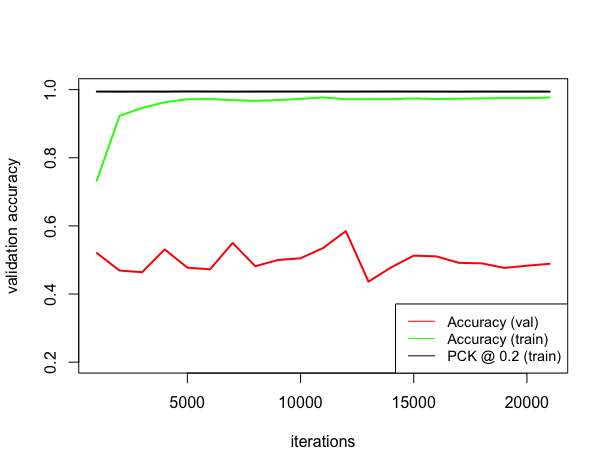
\includegraphics[width=0.8\textwidth]{har_jhmdb_training.png}
        \caption{The training and validation accuracies computed during the training process of the HAR model on JHMDB training data.}
        \end{figure}    
    \begin{itemize}
        \item Best result found in literature: 87.9 percent \footnotemark
    \end{itemize}
    \footnotetext[1]{\cite{choutas_potion:_2018}}
\end{myframe}

\begin{myframe}[End-to-end learning using JHMDB dataset]
    \begin{itemize}
        \item Combining loss functions of pose estimation and HAR
        \item Same model architecture as before
        \item Long training time
    \end{itemize}
    \begin{figure}
        \centering
        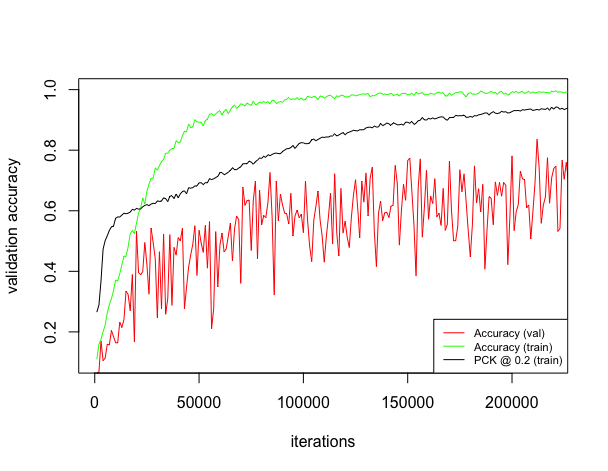
\includegraphics[width=0.8\textwidth]{e2e_big.png}
        \caption{Training and validation accuracies of the HAR model trained using an end-to-end approach, without pretraining individual parts of the model.}
        \label{fig:e2e_big}
    \end{figure}
    
\end{myframe}

\begin{myframe}[End-to-end learning using JHMDB dataset]
    \begin{itemize}
        \item Accuracy significantly worse in comparison to state-of-the-art
        \begin{itemize}
            \item Most likely due to worse pose estimator
        \end{itemize}
        \item Results still promising
        \begin{itemize}
            \item Future work: Architecture changes (see conclusion)
        \end{itemize}
    \end{itemize}
    \begin{table}[]
        \small
        \centering
        \begin{tabular}{|c|c||c|c|}
        \hline
            \textbf{Single Clip accuracy} & \textbf{Multi Clip accuracy}  & \footnotemark[1] & \footnotemark[2] \\ \hline
            65.88 & 68.09 & 78.81 & \textbf{87.90} \\ \hline
        \end{tabular}
        \caption{Test results of the action recognition accuracy on the JHMDB test The accuracy values are much lower in comparison to the state-of-the-art methods.}
        \label{tab:e2e-quantitative-results}
    \end{table}

    \footnotetext[1]{\cite{khalid_multi-modal_2018}}
    \footnotetext[2]{\cite{choutas_potion:_2018}}
    
    \begin{table}[]
        \small
        \centering
        \begin{tabular}{|c|c|c|c|}
            \hline
                & \textbf{PCK @ 0.2} & \textbf{PCK @ 0.1} & \textbf{PCKu @ 0.2}\\ \hline
                End-to-end model & 81.12 & 49.23 & 35.63 \\ \hline
                \begin{tabular}{@{}c@{}} JHMDB pose estimator\\ $4$ prediction blocks, $0$ context heatmaps  \end{tabular}  & \textbf{96.94} & \textbf{91.69} & \textbf{87.49} \\ \hline
            \end{tabular}
            \caption{Pose estimation accuracy, meassured using three different metrics}
            \label{tab:e2e-pose}
    \end{table}
\end{myframe}

\begin{myframe}[End-to-end learning using JHMDB dataset]
    \begin{itemize}
        \item Strong confusion between \textit{sit} and \textit{stand}
        \begin{itemize}
            \item More temporal information architecture might resolve some confusion
        \end{itemize}
    \end{itemize}
    \begin{figure}
        \centering
        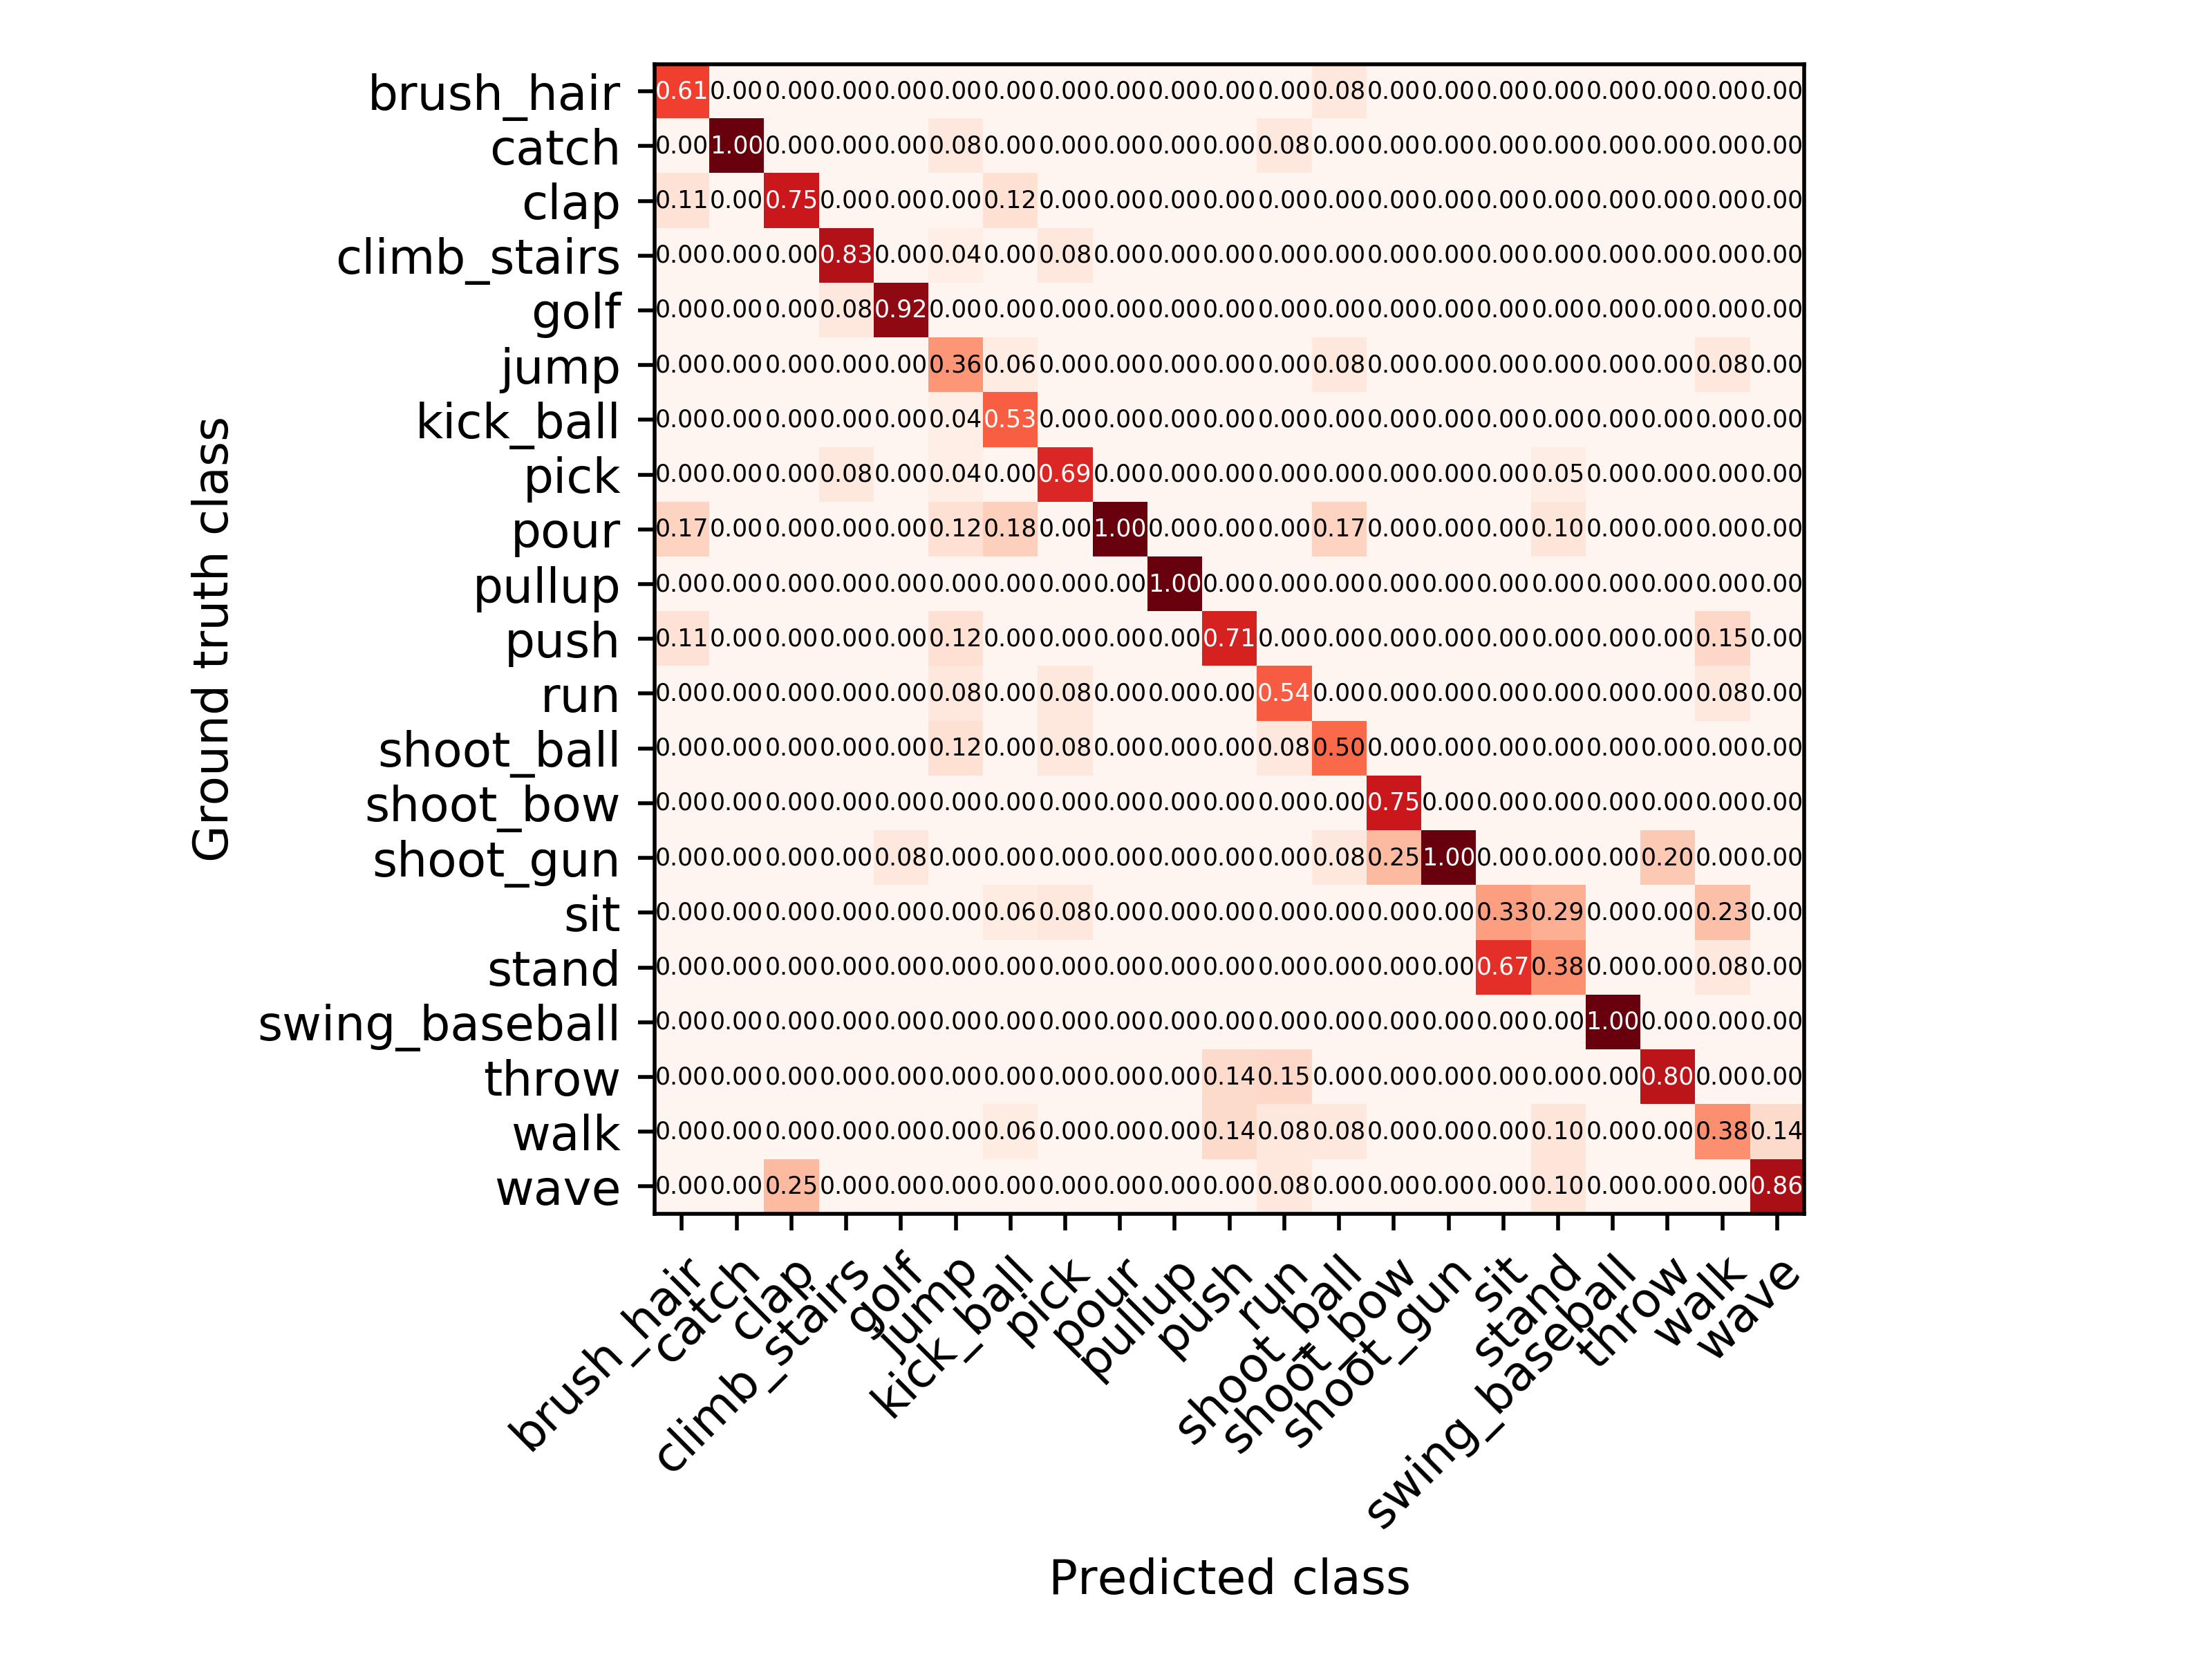
\includegraphics[width=0.999\textwidth]{cm-e2e.png}
        \caption{Confusion matrix, computed on the JHMDB test dataset, using the end-to-end model. Notice the strong confusion between the classes \textit{sit} and \textit{stand}.}
        \label{fig:cm-e2e}
    \end{figure}
\end{myframe}

\section{Conclusion}
\begin{myframe}[Conclusion]
    \begin{itemize}
        \item Results
        \begin{itemize}
            \item Results of \footnotemark[1] could not be recreated exactly
            \item JHMDB HAR model was not able to be trained
            \item Large amount of data necessary to train deep pose estimator (JHMDB too small)
            \item Right side limbs are more accurately detected in comparison to left side limbs
        \end{itemize}
        \item Future work:
        \begin{itemize}
            \item Change model architecture to use a video pose estimator instead of frame-by-frame
            \item More temporal information in architecture (will reduce confusion)
            \item Gather larger, fully annotated video dataset
            \item Right side bias: Due to dataset or architecture?
        \end{itemize}            
    \end{itemize}
    \footnotetext[1]{\cite{luvizon_2d/3d_2018}}
    % \begin{itemize}
    %     \item Stacked architecture in pose estimator increases accuracy until $nr\_blocks = 4$
    %     \item Using context heatmaps does not significantly increase accuracy
    %     \item JHMDB seems to be harder than MPII for pose estimation
    %     \item What will be done next
    %     \begin{itemize}
    %         \item Fine-tuning network once the network is no longer overfitting
    %         \item End-to-end training on JHMDB dataset
    %         \item Evaluate use of different \textit{pose cube} feature extraction
    %     \end{itemize}
    %     \item Future work suggestions
    %     \begin{itemize}
    %         \item Use video pose estimator
    %         \item Gather bigger, fully annotated video datasets for end-to-end Human Activity Recognition
    %     \end{itemize}
    % \end{itemize}
\end{myframe}

\begin{myframe}[Thank you]
    \centering \Large
    \emph{Thank you for your time!}
\end{myframe}

\end{document}

